\chapter{Chemische potentiaal en mengsels}\label{ch:b2:chemical-potential}

In de winter strooit een vrachtwagen zout op een ijzige weg en smelt het ijs bij
\qty{-10}{\celsius}; de koelvloeistof van een automotor, water met een derde
ethaan-1,2-diol, bevriest niet in de nachtvorst en kookt niet onder een hete
motorkap. Een opgeloste stof verlaagt het vriespunt van haar oplosmiddel en
verhoogt het kookpunt ervan, en voor verdunde oplossingen met een bedrag dat
afhangt van het aantal opgeloste deeltjes en niet van hun aard. Het
werktuig dat dit verklaart, is de \omterm{def:b2:chemical-potential:chemical-potential}{chemische potentiaal}, de partiële afgeleide van
de \omterm{def:b2:reaction-free-energy:gibbs-energy}{gibbsenergie} naar de hoeveelheid van één bestanddeel. Ze zegt
waar elk deeltje ``naartoe wil'', tussen fasen en via reacties,
en ze maakt van de activiteiten, die het deel van jaar~1 als recepten gebruikte,
afgeleide grootheden.

\begin{recall}
\Cref{ch:b2:reaction-free-energy}: de \omterm{def:b2:reaction-free-energy:gibbs-energy}{gibbsenergie} $G = H - TS$, $\dd G =
V\dd p - S\dd T + \Delta_r G\,\dd\xi$, het evolutiecriterium $\Delta_r G\,
\dd\xi \leq 0$. Het deel van jaar~1 schreef de activiteit van een gas als
$p_i/p^\circ$, van een opgeloste stof als $c_i/c^\circ$, en 1 voor een zuivere vaste stof of een
oplosmiddel, en merkte op dat activiteiten in geconcentreerde ionaire oplossingen afwijken
van concentraties, ``een correctie die in het deel van jaar~2 behandeld wordt''. Uit
de natuurkunde: de ideale gaswet, en $(\partial G/\partial p)_T = V$ voor een zuivere
stof.
\end{recall}

\begin{omfigure}

\includegraphics[width=0.58\linewidth]{images/book3/ai/b2-03-salt-spreader.jpg}

{\small Een strooiwagen strooit zout op een besneeuwde weg. Het zout lost op
in het dunne waterlaagje op het ijs, en de oplossing bevriest bij een lagere
temperatuur dan zuiver water: het ijs smelt.}
\end{omfigure}

\section{Partiële molaire grootheden}

Meng \qty{50}{mL} water en \qty{50}{mL} ethanol: het volume van het
mengsel is kleiner dan \qty{100}{mL}. In een mengsel is een extensieve grootheid
niet de som van de bijdragen van de zuivere stoffen; elk bestanddeel
draagt bij naargelang zijn omgeving.

\begin{definition}[Partiële molaire grootheid]\label{def:b2:chemical-potential:partial-molar}
Zij $X(T, p, n_1, \dots, n_k)$ een extensieve toestandsfunctie van een fase
die de hoeveelheden $n_1, \dots, n_k$ bevat. De \emph{partiële molaire
grootheid}\index{partiele molaire grootheid@partiële molaire grootheid} van bestanddeel $i$ is
\[
  \bar X_i = \left(\frac{\partial X}{\partial n_i}\right)_{T, p, n_{j \ne i}} ,
\]
de verandering van $X$ per mol $i$ die aan een grote hoeveelheid mengsel wordt toegevoegd,
bij vaste $T$, $p$ en overige hoeveelheden. Voor $X = V$ is dat het \emph{partieel
molair volume}\index{partieel molair volume} $\bar V_i$.
\end{definition}

\begin{theorem}[Identiteit van Euler]\label{thm:b2:chemical-potential:euler}
Bij vaste $T$ en $p$ is $X = \sum_i n_i\bar X_i$.
\end{theorem}

\begin{proof}
$X$ is extensief: alle hoeveelheden met $\lambda$ vermenigvuldigen vermenigvuldigt $X$ met
$\lambda$, $X(T, p, \lambda n_1, \dots, \lambda n_k) = \lambda X(T, p, n_1,
\dots, n_k)$. Differentieer naar $\lambda$ in $\lambda = 1$, met
de kettingregel: $\sum_i n_i\,\partial X/\partial n_i = X$.
\end{proof}

\begin{proposition}[Betrekking van Gibbs--Duhem]\label{prop:b2:chemical-potential:gibbs-duhem}
Bij vaste $T$ en $p$ is $\sum_i n_i\,\dd\bar X_i = 0$: in een binair mengsel
geldt $x_1\dd\bar X_1 + x_2\dd\bar X_2 = 0$. De partiële molaire grootheden van de
bestanddelen kunnen niet onafhankelijk variëren.
\end{proposition}

\begin{proof}
Bij vaste $T$, $p$ is per definitie $\dd X = \sum_i\bar X_i\dd n_i$; de identiteit
van Euler, gedifferentieerd, geeft $\dd X = \sum_i\bar X_i\dd n_i + \sum_i
n_i\dd\bar X_i$. Trek af.
\end{proof}

\begin{omfigure}
\begin{tikzpicture}
\begin{axis}[
  width=0.62\linewidth, height=5.4cm, xmin=0, xmax=1, ymin=8, ymax=62,
  axis x line=bottom, axis y line=left, xlabel={molfractie $x_2$},
  ylabel={molair volume $V_m$ (model)}, xtick={0,0.2,0.4,0.6,0.8,1}, ytick=\empty,
  tick label style={font=\small}, label style={font=\small}, ylabel shift=10pt, clip=false]
\addplot[omDef, very thick, domain=0:1, samples=60] {18*(1-x) + 58*x - 25*x*(1-x)};
\addplot[black!40, dashed, domain=0:1] {18*(1-x) + 58*x};
\addplot[omThm, thick, domain=0:1] {14 + 35*x};
\fill[omThm] (axis cs:0.4,28) circle (1.6pt);
\node[omThm, anchor=east, font=\small] at (axis cs:-0.01,14) {$\bar V_1$};
\node[omThm, anchor=west, font=\small] at (axis cs:1,49) {$\bar V_2$};
\node[font=\scriptsize, anchor=south east, black!60] at (axis cs:0.62,44) {zuivere volumes opgeteld};
\node[font=\small, anchor=north west] at (axis cs:0.41,27) {$x_2 = 0.4$};
\end{axis}
\end{tikzpicture}

{\small De raaklijnconstructie. Het molair volume van een binair modelmengsel
(blauw) ligt onder de rechte die de zuivere volumes verbindt: mengen
doet krimpen. De raaklijn bij een samenstelling snijdt de twee randen in de partiële
molaire volumes $\bar V_1$ en $\bar V_2$ bij die samenstelling.}
\end{omfigure}

\begin{method}[Partiële molaire grootheden uit een kromme]\label{met:b2:chemical-potential:tangent}
Zet de molaire grootheid $X_m = X/(n_1 + n_2)$ uit tegen $x_2$. Teken bij de
samenstelling die je zoekt de raaklijn: ze snijdt de as $x_2 = 0$ in
$\bar X_1$ en de as $x_2 = 1$ in $\bar X_2$. (Bewijs: $X_m = x_1\bar X_1 +
x_2\bar X_2$ en, volgens Gibbs--Duhem, $\dd X_m/\dd x_2 = \bar X_2 - \bar X_1$.)
\end{method}

\section{De chemische potentiaal}

\begin{definition}[Chemische potentiaal]\label{def:b2:chemical-potential:chemical-potential}
De \emph{chemische potentiaal}\index{chemische potentiaal} van bestanddeel $i$ in
een fase is zijn partiële molaire \omterm{def:b2:reaction-free-energy:gibbs-energy}{gibbsenergie},
\[
  \mu_i = \left(\frac{\partial G}{\partial n_i}\right)_{T, p, n_{j\ne i}} ,
\]
in \unit{J/mol}. Haar waarde wanneer $i$ in zijn standaardtoestand is, is zijn
\emph{standaard chemische potentiaal}\index{standaard chemische potentiaal}
$\mu_i^\circ(T)$, gelijk aan de molaire standaardgibbsenergie van $i$.
\end{definition}

Voor een fase waarvan de hoeveelheden kunnen veranderen (door reactie, of door uitwisseling met
een andere fase) geldt
\[
  \dd G = V\dd p - S\dd T + \sum_i\mu_i\,\dd n_i ,\qquad G = \sum_i n_i\mu_i ,
\]
de tweede betrekking volgens de identiteit van Euler. Met één enkele reactie is $\dd n_i =
\nu_i\dd\xi$, en vergelijken met \cref{prop:b2:reaction-free-energy:dG} geeft
\[
  \Delta_r G = \sum_i\nu_i\mu_i .
\]
De \omterm{def:b2:reaction-free-energy:reaction-gibbs}{reactie-gibbsenergie} is de balans van de \omterm{def:b2:chemical-potential:chemical-potential}{chemische potentialen} van de
reactieproducten en van de beginstoffen.

\begin{theorem}[Evenwicht tussen fasen]\label{thm:b2:chemical-potential:phase-equilibrium}
Een bestanddeel dat aanwezig is in twee fasen $\alpha$ en $\beta$ van een gesloten systeem bij
uniforme $T$ en $p$, is tussen die fasen in evenwicht dan en slechts dan als
$\mu_i^\alpha = \mu_i^\beta$. Anders gaat het spontaan over van de
fase waarin zijn \omterm{def:b2:chemical-potential:chemical-potential}{chemische potentiaal} hoger is naar de fase waarin ze lager is.
\end{theorem}

\begin{proof}
De overdracht $i^\alpha \to i^\beta$ is een ``reactie'' met $\nu^\alpha = -1$,
$\nu^\beta = +1$, dus $\Delta_r G = \mu_i^\beta - \mu_i^\alpha$. Volgens het
evolutiecriterium schrijdt ze alleen voort ($\dd\xi > 0$) als $\mu_i^\beta <
\mu_i^\alpha$, loopt ze terug als $\mu_i^\beta > \mu_i^\alpha$, en is ze in
evenwicht als beide gelijk zijn.
\end{proof}

De \omterm{def:b2:chemical-potential:chemical-potential}{chemische potentiaal} speelt voor materie de rol die de temperatuur speelt
voor warmte: warmte stroomt van warm naar koud, een deeltje van hoge naar lage $\mu$.

\section{Ideale systemen en activiteiten}

\begin{proposition}[Chemische potentiaal van een ideaal gas]\label{prop:b2:chemical-potential:mu-gas}
In een mengsel van ideale gassen heeft een gas met partiële druk $p_i$
\[
  \mu_i = \mu_i^\circ(T) + RT\ln\frac{p_i}{p^\circ} .
\]
\end{proposition}

\begin{proof}
Voor één mol van een zuiver ideaal gas is $(\partial\mu/\partial p)_T = V_m =
RT/p$; integreren van $p^\circ$ tot $p$ geeft $\mu = \mu^\circ + RT\ln(p/p^\circ)$.
In een mengsel van ideale gassen gedraagt elk gas zich alsof het alleen in het volume is, bij
zijn partiële druk: vervang $p$ door $p_i$.
\end{proof}

\begin{definition}[Ideaal mengsel, ideaal verdunde oplossing]\label{def:b2:chemical-potential:ideal-mixture}
Een vloeibaar (of vast) mengsel is een \emph{ideaal mengsel}\index{ideaal mengsel}
als voor elk bestanddeel en elke samenstelling
$\mu_i = \mu_i^*(T, p) + RT\ln x_i$, waarin $\mu_i^*$ de \omterm{def:b2:chemical-potential:chemical-potential}{chemische potentiaal}
van de zuivere vloeistof $i$ is. Een oplossing is een \emph{ideaal verdunde
oplossing}\index{ideaal verdunde oplossing} als het oplosmiddel deze wet volgt en elke
opgeloste stof $\mu_j = \mu_j^\circ(T) + RT\ln(c_j/c^\circ)$ volgt, met als
standaardtoestand een hypothetische oplossing bij $c^\circ = \qty{1}{mol/L}$ die zich gedraagt
alsof ze oneindig verdund is.
\end{definition}

Moleculen van vergelijkbare grootte en vorm waarvan de interacties niet van de
partner afhangen (benzeen en tolueen, twee isotopische vormen van een molecuul), vormen
bijna ideale mengsels; verdunde oplossingen gedragen zich ideaal omdat elk opgelost
deeltje alleen door oplosmiddel omringd is.

\begin{theorem}[Wet van Raoult]\label{thm:b2:chemical-potential:raoult}
Boven een ideaal vloeibaar mengsel, met de damp als ideaal gas, is de partiële
druk van elk bestanddeel evenredig met zijn molfractie in de
vloeistof: $p_i = x_i\,p_i^*$, waarin $p_i^*$ de dampdruk is van de zuivere
vloeistof bij dezelfde temperatuur (\emph{wet van Raoult}\index{wet van Raoult}).
\end{theorem}

\begin{proof}
In evenwicht is $\mu_i(\text{vloeistof}) = \mu_i(\text{damp})$: $\mu_i^* +
RT\ln x_i = \mu_i^\circ + RT\ln(p_i/p^\circ)$. Voor de zuivere vloeistof ($x_i = 1$,
$p_i = p_i^*$): $\mu_i^* = \mu_i^\circ + RT\ln(p_i^*/p^\circ)$. Aftrekken geeft
$RT\ln x_i = RT\ln(p_i/p_i^*)$. (De zwakke afhankelijkheid van $\mu_i^*$ van de
druk wordt verwaarloosd.)
\end{proof}

\begin{proposition}[Wet van Henry]\label{prop:b2:chemical-potential:henry}
Voor een verdunde opgeloste stof $j$ in evenwicht met haar damp geldt $p_j = k_{H,j}\,x_j$
(of $c_j = H_j\,p_j$): de partiële druk van een verdunde opgeloste stof is
evenredig met haar hoeveelheid in de oplossing (\emph{wet van
Henry}\index{wet van Henry}). De \emph{henryconstante}\index{henryconstante}
$k_{H,j}$ hangt af van de opgeloste stof, het oplosmiddel en de temperatuur, en is niet
de dampdruk van de zuivere opgeloste stof.
\end{proposition}

\begin{proof}
Stel $\mu_j^\circ(\text{oplossing}) + RT\ln(c_j/c^\circ)$ en
$\mu_j^\circ(\text{gas}) + RT\ln(p_j/p^\circ)$ gelijk: $c_j/p_j$ is een functie van alleen
$T$. De constante bevat de interacties van $j$ met het oplosmiddel, niet
met zichzelf.
\end{proof}

\begin{omfigure}
\begin{tikzpicture}
\begin{axis}[name=a,
  width=0.48\linewidth, height=5.6cm, xmin=0, xmax=1, ymin=0, ymax=1.5,
  axis x line=bottom, axis y line=left, xlabel={$x_1$}, ylabel={$p/p_1^*$},
  xtick={0,0.5,1}, ytick={0,0.5,1,1.5},
  tick label style={font=\small}, label style={font=\small}, title={\small ideaal}]
\addplot[omDef, thick] table[x=x1, y=p1] {figdata/out/bachelor-2-raoult-henry-ideal.dat};
\addplot[omThm, thick] table[x=x1, y=p2] {figdata/out/bachelor-2-raoult-henry-ideal.dat};
\addplot[black, very thick] table[x=x1, y=p] {figdata/out/bachelor-2-raoult-henry-ideal.dat};
\node[omDef, font=\scriptsize, anchor=west] at (axis cs:0.55,0.42) {$p_1$};
\node[omThm, font=\scriptsize, anchor=west] at (axis cs:0.1,0.42) {$p_2$};
\node[font=\scriptsize, anchor=south] at (axis cs:0.5,0.8) {$p$};
\end{axis}
\begin{axis}[at={(a.east)}, anchor=west, xshift=1.2cm,
  width=0.48\linewidth, height=5.6cm, xmin=0, xmax=1, ymin=0, ymax=1.5,
  axis x line=bottom, axis y line=left, xlabel={$x_1$},
  xtick={0,0.5,1}, ytick={0,0.5,1,1.5},
  tick label style={font=\small}, label style={font=\small}, title={\small positieve afwijking}]
\addplot[omDef, thick] table[x=x1, y=p1] {figdata/out/bachelor-2-raoult-henry-margules.dat};
\addplot[omThm, thick] table[x=x1, y=p2] {figdata/out/bachelor-2-raoult-henry-margules.dat};
\addplot[black, very thick] table[x=x1, y=p] {figdata/out/bachelor-2-raoult-henry-margules.dat};
\addplot[omDef, densely dashed, domain=0.6:1] {x};
\addplot[omDef, dotted, thick, domain=0:0.42] {3.004166*x};
\node[omDef, font=\scriptsize, anchor=west] at (axis cs:0.62,0.5) {Raoult};
\node[omDef, font=\scriptsize, anchor=east] at (axis cs:0.27,1.18) {Henry};
\node[omDef, font=\scriptsize, anchor=north west] at (axis cs:0.8,0.78) {$p_1$};
\node[omThm, font=\scriptsize, anchor=north] at (axis cs:0.55,0.24) {$p_2$};
\node[font=\scriptsize, anchor=south] at (axis cs:0.5,1.23) {$p$};
\end{axis}
\end{tikzpicture}

{\small Dampdrukken boven een binaire vloeistof bij vaste temperatuur, in eenheden
van $p_1^*$ (modelmengsel). Links een \omterm{def:b2:chemical-potential:ideal-mixture}{ideaal mengsel}: rechte lijnen (Raoult).
Rechts een mengsel waarin ongelijke moleculen elkaar minder aantrekken dan gelijke:
de drukken liggen boven de ideale lijnen. Dicht bij $x_1 = 1$ volgt bestanddeel 1
de lijn van Raoult (gestreept); dicht bij $x_1 = 0$ volgt het een lijn van Henry
(gestippeld) met een andere helling.}
% (computed in figdata/bachelor-2/raoult-henry.py; Margules parameter 1.1, model)
\end{omfigure}

\begin{example}[Koolstofdioxide in frisdrank]\label{ex:b2:chemical-potential:soda}
Bij \qty{25}{\celsius} is de \omterm{prop:b2:chemical-potential:henry}{henryconstante} van koolstofdioxide in water $H =
\qty{3.4e-4}{mol/(m^3.Pa)}$, dat is \qty{0.034}{mol/(L.bar)}. Een fles die
onder \qty{4}{bar} \ce{CO2} is afgesloten, bevat $0.034 \times 4 =
\qty{0.14}{mol/L}$ opgelost gas, ongeveer \qty{6}{g/L}. Na het openen is het gas
erboven de lucht, waarin $p_{\ce{CO2}} \approx \qty{4e-4}{bar}$: de drank is
tienduizendvoudig oververzadigd en bruist tot hij verschaald is.
% ledger: henry:CO2, air:CO2
\end{example}

\begin{proposition}[Activiteiten uit chemische potentialen]\label{prop:b2:chemical-potential:activity}
In elk tot nu toe besproken geval is $\mu_i = \mu_i^\circ(T) + RT\ln a_i$, waarin $a_i$
de activiteit van het deel van jaar~1 is: $p_i/p^\circ$ voor een ideaal gas,
$c_i/c^\circ$ voor een opgeloste stof in een \omterm{def:b2:chemical-potential:ideal-mixture}{ideaal verdunde oplossing}, $x_i$ (dicht bij 1)
voor het oplosmiddel, en 1 voor een zuivere vaste stof of vloeistof alleen in haar fase.
\end{proposition}

\begin{proof}
Voor het gas en de verdunde opgeloste stof is dit de inhoud van
\cref{prop:b2:chemical-potential:mu-gas} en van de definitie van de \omterm{def:b2:chemical-potential:ideal-mixture}{ideaal
verdunde oplossing}. Neem voor een bestanddeel van een \omterm{def:b2:chemical-potential:ideal-mixture}{ideaal mengsel} de zuivere
vloeistof als standaardtoestand: $a_i = x_i$, dicht bij 1 voor een oplosmiddel. Een zuivere vaste stof
of vloeistof is haar eigen standaardtoestand (haar zwakke afhankelijkheid van de druk
verwaarloosd): $\mu = \mu^\circ$, $a = 1$.
\end{proof}

\begin{proposition}[Reactie-gibbsenergie en reactiequotiënt]\label{prop:b2:chemical-potential:delta-g-q}
Voor een reactie $0 = \sum_i\nu_i\mathrm A_i$ geldt
\[
  \Delta_r G = \Delta_r G^\circ(T) + RT\ln Q, \qquad Q = \prod_i a_i^{\nu_i} .
\]
\end{proposition}

\begin{proof}
$\Delta_r G = \sum_i\nu_i\mu_i = \sum_i\nu_i\mu_i^\circ + RT\sum_i\nu_i\ln a_i =
\Delta_r G^\circ + RT\ln\prod_i a_i^{\nu_i}$.
\end{proof}

Dit is de brug tussen de \omterm{def:b2:reaction-free-energy:gibbs-energy}{gibbsenergie} van \cref{ch:b2:reaction-free-energy}
en het reactiequotiënt van het deel van jaar~1. Het volgende hoofdstuk steekt haar over.

\begin{method}[De referentietoestand van een activiteit kiezen]\label{met:b2:chemical-potential:activity-reference}
\begin{enumerate}
  \item Gas: het zuivere ideale gas bij $p^\circ$; $a = p_i/p^\circ$.
  \item Oplosmiddel, of een bestanddeel van een mengsel met vergelijkbare hoeveelheden: de
        zuivere vloeistof; $a = \gamma_i x_i$ (referentie van Raoult, $\gamma_i \to 1$
        als $x_i \to 1$).
  \item Opgeloste stof: de ideale oplossing bij $c^\circ$; $a = \gamma_j c_j/c^\circ$
        (referentie van Henry, $\gamma_j \to 1$ bij oneindige verdunning).
  \item Zuivere vaste stof, zuivere vloeistof alleen in haar fase: $a = 1$.
\end{enumerate}
\end{method}

\begin{history}[François-Marie Raoult]
\begin{minipage}[t]{0.2\linewidth}\vspace{0pt}
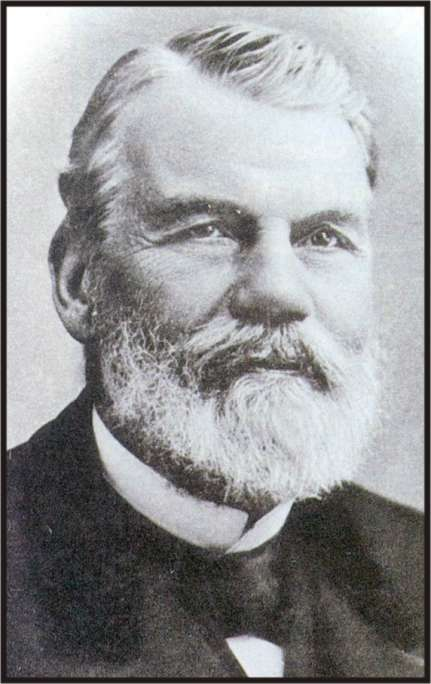
\includegraphics[width=\linewidth]{images/book3/raoult.jpg}
\end{minipage}\hfill
\begin{minipage}[t]{0.76\linewidth}\vspace{0pt}
François-Marie Raoult (1830--1901), hoogleraar scheikunde in Grenoble,
mat in de jaren 1880 de vriespunten en daarna de dampdrukken
van honderden oplossingen, en vond dat de verlaging voor verdunde oplossingen
afhangt van het aantal opgeloste moleculen en niet van hun aard. Zijn
metingen werden een manier om moleculen te wegen, en ondersteunden de jonge
theorie van ionen in oplossing. (Foto: publiek domein, Wikimedia Commons.)
\end{minipage}
\end{history}

\section{Reële mengsels}

\begin{definition}[Activiteitscoëfficiënt]\label{def:b2:chemical-potential:activity-coefficient}
In een reëel mengsel wordt de \omterm{def:b2:chemical-potential:chemical-potential}{chemische potentiaal} geschreven als $\mu_i = \mu_i^\circ +
RT\ln a_i$ met $a_i = \gamma_i x_i$ (referentie van Raoult) of $a_i = \gamma_i
c_i/c^\circ$ (referentie van Henry). De factor $\gamma_i$ is de
\emph{activiteitscoëfficiënt}\index{activiteitscoefficient@activiteitscoëfficiënt}: hij meet de afwijking van de
ideale wet, en gaat naar 1 in de limiet waarin de referentiewet geldt.
\end{definition}

Een coëfficiënt groter dan 1 betekent dat het molecuul in het mengsel door zijn
buren minder gestabiliseerd wordt dan in de referentietoestand (positieve afwijking, zoals in de figuur
hierboven); kleiner dan 1, meer gestabiliseerd. Volgens Gibbs--Duhem zijn de coëfficiënten van de twee
bestanddelen van een binair mengsel gekoppeld: in het model met één parameter
dat voor de figuur gebruikt is, geldt $\ln\gamma_1 = Ax_2^2$ en $\ln\gamma_2 = Ax_1^2$, en
$x_1\,\dd\ln\gamma_1 + x_2\,\dd\ln\gamma_2 = 0$ is identiek voldaan.

Voor ionen, die op lange afstand wisselwerken, verschijnen afwijkingen al bij kleine
concentraties.

\begin{definition}[Ionsterkte]\label{def:b2:chemical-potential:ionic-strength}
De \emph{ionsterkte}\index{ionsterkte} van een oplossing is $I =
\frac12\sum_i z_i^2\,b_i$, waarin $b_i$ de molaliteit van ion $i$ is (hoeveelheid per
kilogram oplosmiddel) en $z_i$ zijn ladingsgetal.
\end{definition}

\begin{proposition}[Grenswet van Debye--Hückel]\label{prop:b2:chemical-potential:debye-huckel}
In een zeer verdunde elektrolytoplossing volgt de gemiddelde \omterm{def:b2:chemical-potential:activity-coefficient}{activiteitscoëfficiënt} van de
ionen van een zout $\log\gamma_\pm = -A\,|z_+z_-|\sqrt{I/b^\circ}$, met $A
\approx 0.51$ voor water bij \qty{25}{\celsius} en $b^\circ =
\qty{1}{mol/kg}$.
\end{proposition}
\admitted

\begin{remark}[Geldigheid en oorsprong]\label{rem:b2:chemical-potential:dh-range}
De wet komt uit een model waarin elk ion omringd is door een diffuse
``atmosfeer'' van tegengestelde lading, die zijn \omterm{def:b2:chemical-potential:chemical-potential}{chemische potentiaal} verlaagt; het
model valt buiten deze cursus, maar de constante $A$ volgt uit de
permittiviteit en de dichtheid van water en de temperatuur. De wet is nauwkeurig onder
ongeveer $I = \qty{0.01}{mol/kg}$. Dezelfde ionenatmosfeer remt de ionen in
een elektrisch veld af, en verklaart waarom de molaire geleidbaarheid van een sterke
elektrolyt daalt als $\Lambda = \Lambda^\circ - K\sqrt c$ (wortelwet van
Kohlrausch) in plaats van op haar grenswaarde te blijven: de grens van de
wet van Kohlrausch die in het deel van jaar~1 aan bod kwam.
% ledger: epsr:H2O, rho:water.298, const:e, const:eps0, const:kB, const:NA (A computed in figdata/bachelor-2/colligative.py)
\end{remark}

\begin{example}[Een centimolair zout]\label{ex:b2:chemical-potential:dh}
Voor natriumchloride bij $b = \qty{0.010}{mol/kg}$ is $I = \frac12(0.010 + 0.010)
= \qty{0.010}{mol/kg}$ en $\log\gamma_\pm = -0.51 \times 0.10$: $\gamma_\pm
= 0.89$. Al bij een honderdste mol per kilogram is het gelijkstellen van
concentratie en activiteit een fout van 11\,\%; voor een 2:2-zout zoals
magnesiumsulfaat bij dezelfde molaliteit is $I = 0.040$ en $\gamma_\pm = 0.62$.
\end{example}

\section{Colligatieve eigenschappen}

\begin{definition}[Colligatieve eigenschap]\label{def:b2:chemical-potential:colligative}
Een \emph{colligatieve eigenschap}\index{colligatieve eigenschap} van een verdunde
oplossing hangt af van de hoeveelheid opgeloste deeltjes per
hoeveelheid oplosmiddel en niet van hun aard: de verlaging van de dampdruk
en van het vriespunt, de verhoging van het kookpunt, en de
\omterm{def:b2:chemical-potential:osmotic-pressure}{osmotische druk}. De constanten van de vriespunts- en kookpuntswetten
hieronder zijn de \emph{cryoscopische constante}\index{cryoscopische constante} $K_f$
en de \emph{ebullioscopische constante}\index{ebullioscopische constante} $K_b$ van
het oplosmiddel.
\end{definition}

\begin{omfigure}
\begin{tikzpicture}[font=\small, >={Stealth}]
  \draw[->] (0,0) -- (8,0) node[right] {$T$};
  \draw[->] (0,0) -- (0,4.4) node[above] {$\mu$ van het oplosmiddel};
  % slopes = -S_m: the liquid, more disordered, falls faster than the solid
  \draw[omDef, very thick] (0.4,3.0) -- (7.0,2.01) node[right] {vaste stof};
  \draw[omThm, very thick] (0.4,3.6) -- (7.6,0.72) node[right] {zuivere vloeistof};
  \draw[omThm, very thick, dashed] (0.4,3.25) -- (7.6,0.37) node[right] {oplossing};
  \fill (2.8,2.64) circle (1.5pt);
  \fill (1.4,2.85) circle (1.5pt);
  \draw[densely dotted] (2.8,2.64) -- (2.8,0) node[below] {$T_f^*$};
  \draw[densely dotted] (1.4,2.85) -- (1.4,0) node[below] {$T_f$};
  \draw[<->] (1.4,-0.75) -- (2.8,-0.75) node[midway, below] {$\Delta T_f$};
  \draw[<->, black!70] (5.0,1.76) -- (5.0,1.41);
  \draw[black!50] (5.0,1.58) -- (4.6,0.75) node[below, font=\scriptsize, black] {$RT\ln x_1$};
\end{tikzpicture}

{\small \omterm{def:b2:chemical-potential:chemical-potential}{Chemische potentiaal} van het oplosmiddel als functie van de temperatuur (schematisch,
bij vaste druk). De stabiele fase is die met de laagste $\mu$. Het oplossen van een
stof verlaagt de lijn van de vloeistof met $RT\ln x_1 < 0$; ze snijdt de lijn van de vaste stof
nu bij een lagere temperatuur: de oplossing bevriest onder het zuivere oplosmiddel.}
\end{omfigure}

\begin{theorem}[Vriespuntsdaling]\label{thm:b2:chemical-potential:cryoscopy}
Een verdunde oplossing van een stof die niet in de vaste fase opgenomen wordt, begint te bevriezen
bij $T_f = T_f^* - \Delta T_f$, met
\[
  \Delta T_f = K_f\,b, \qquad K_f = \frac{R\,T_f^{*2}\,M_1}{\Delta_{\text{fus}}H_1} ,
\]
waarin $b$ de totale molaliteit van de opgeloste deeltjes is en $M_1$ de molaire
massa van het oplosmiddel (in \unit{kg/mol}). Voor eindige concentraties is de exacte
betrekking voor een ideale oplossing $\ln x_1 = -\frac{\Delta_{\text{fus}}H_1}{R}
\left(\frac{1}{T_f} - \frac{1}{T_f^*}\right)$.
\end{theorem}

\begin{proof}
Bij het vriespunt zijn het zuivere vaste oplosmiddel en het oplosmiddel in de oplossing in
evenwicht: $\mu_1^{\text{s}}(T) = \mu_1^{*\text{l}}(T) + RT\ln x_1$, dus
$\ln x_1 = -\Delta_{\text{fus}}G_1(T)/(RT)$, met $\Delta_{\text{fus}}G_1 =
\mu_1^{*\text{l}} - \mu_1^{\text{s}}$, nul bij $T_f^*$. Volgens Gibbs--Helmholtz is
$\dd(\Delta_{\text{fus}}G_1/T)/\dd T = -\Delta_{\text{fus}}H_1/T^2$;
integreren van $T_f^*$ tot $T_f$ met constante $\Delta_{\text{fus}}H_1$ geeft
de exacte betrekking. Voor een verdunde oplossing is $\ln x_1 = \ln(1 - x_2) \approx
-x_2$ en $\frac1{T_f} - \frac1{T_f^*} \approx -\Delta T_f/T_f^{*2}$, dus
$x_2 = \Delta_{\text{fus}}H_1\Delta T_f/(RT_f^{*2})$; ten slotte is $x_2 \approx
n_2/n_1 = b\,M_1$.
\end{proof}

\begin{proposition}[Kookpuntsverhoging]\label{prop:b2:chemical-potential:ebullioscopy}
Een verdunde oplossing van een niet-vluchtige stof kookt bij $T_b^* + \Delta T_b$ met
$\Delta T_b = K_b\,b$, $K_b = RT_b^{*2}M_1/\Delta_{\text{vap}}H_1$.
\end{proposition}

\begin{proof}
Hetzelfde, met de damp in plaats van de vaste stof: $\mu_1^{*\text{l}} +
RT\ln x_1 = \mu_1^{\text{v}}$; de lijn van het oplosmiddel is verlaagd en snijdt
de lijn van de damp nu bij een hogere temperatuur.
\end{proof}

\begin{example}[Water]\label{ex:b2:chemical-potential:water-constants}
Met $\Delta_{\text{fus}}H = \qty{333.4}{J/g} = \qty{6.007}{kJ/mol}$ bij
\qty{273.15}{K}: $K_f = 8.314 \times 273.15^2 \times 0.018015/6007 =
\qty{1.86}{K.kg/mol}$. Met $\Delta_{\text{vap}}H = \qty{40.65}{kJ/mol}$ bij
\qty{373.12}{K}: $K_b = \qty{0.513}{K.kg/mol}$. Zeewater, \qty{35}{g} zout
per kilogram, gerekend als natriumchloride (twee deeltjes per formule-eenheid):
$b = 2 \times 35/58.44/0.965 = \qty{1.24}{mol/kg}$, dus de verdunde wet
voorspelt \qty{-2.3}{\celsius}, een overschatting: bij deze concentratie zijn de
ionen verre van ideaal, en zeezout is niet uitsluitend natriumchloride.
% ledger: dfus:H2O, tfus:H2O, dvap:H2O.nbp, tb:H2O.atm, sea:salinity (computed in figdata/bachelor-2/colligative.py)
\end{example}

\begin{definition}[Semipermeabel membraan, osmotische druk]\label{def:b2:chemical-potential:osmotic-pressure}
Een \emph{semipermeabel membraan}\index{semipermeabel membraan} laat het
oplosmiddel door en de opgeloste stof niet. Wanneer het een oplossing scheidt van het
zuivere oplosmiddel, stroomt het oplosmiddel de oplossing in; de \emph{osmotische
druk}\index{osmotische druk} $\Pi$ is de overdruk die op de oplossing moet worden
uitgeoefend om die stroming te stoppen.
\end{definition}

\begin{theorem}[Osmotische wet van Van 't Hoff]\label{thm:b2:chemical-potential:osmosis}
Voor een verdunde oplossing is $\Pi = c\,RT$, waarin $c$ de totale concentratie
opgeloste deeltjes is.
\end{theorem}

\begin{proof}
Bij evenwicht heeft het oplosmiddel aan weerszijden dezelfde \omterm{def:b2:chemical-potential:chemical-potential}{chemische potentiaal}:
$\mu_1^*(T, p) = \mu_1^*(T, p + \Pi) + RT\ln x_1$. Omdat $(\partial\mu_1^*/
\partial p)_T = V_{m,1}$, voor een vloeistof bijna constant, is $\mu_1^*(T, p + \Pi) -
\mu_1^*(T, p) = \Pi V_{m,1}$, dus $\Pi V_{m,1} = -RT\ln x_1 \approx RT x_2
\approx RT\,n_2/n_1$. Met $n_1V_{m,1} \approx V$ (verdund) is $\Pi = n_2RT/V$.
\end{proof}

\begin{omfigure}
\begin{tikzpicture}[font=\small, >={Stealth}]
  \begin{scope}
    \clip (-0.85,2.8) -- (-0.85,0.85) arc[start angle=180, end angle=360,
      radius=0.85] -- (0.85,2.8) -- (0.55,2.8) -- (0.55,0.85)
      arc[start angle=0, end angle=-180, radius=0.55] -- (-0.55,2.8) -- cycle;
    \fill[omDef!18] (-1,0) rectangle (0,1.6);
    \fill[omThm!22] (0,0) rectangle (1,2.3);
  \end{scope}
  \pic at (0,0) {utube={0}{white}};
  \draw[very thick, dashed] (0,-0.05) -- (0,0.36);
  \node[left] at (-1.0,1.2) {zuiver water};
  \node[right] at (1.0,0.9) {oplossing};
  \draw[densely dotted] (-0.55,1.6) -- (1.55,1.6);
  \draw[densely dotted] (0.85,2.3) -- (1.55,2.3);
  \draw[<->, thick] (1.45,1.6) -- (1.45,2.3) node[midway, right] {$h$, met $\Pi = \rho g h$};
  \draw (0,0.12) -- (0.6,-0.5) node[below right] {semipermeabel membraan};
  \draw[->, omDef, thick] (-0.75,0.4) to[bend right=30] (-0.25,0.12);
\end{tikzpicture}

{\small Osmose in een U-buis. Water gaat door het membraan de
oplossing in tot de extra hydrostatische druk van de hogere kolom gelijk is aan
de \omterm{def:b2:chemical-potential:osmotic-pressure}{osmotische druk}; dan zijn de \omterm{def:b2:chemical-potential:chemical-potential}{chemische potentialen} van water aan beide kanten
gelijk.}
\end{omfigure}

\begin{method}[Molaire massa via een colligatieve eigenschap]\label{met:b2:chemical-potential:molar-mass}
\begin{enumerate}
  \item Los een bekende massa $m_2$ van de stof op in een bekende massa $m_1$
        oplosmiddel (of een bekend volume $V$ oplossing).
  \item Meet $\Delta T_f$ (of $\Delta T_b$, of $\Pi$).
  \item Leid de molaliteit $b = \Delta T_f/K_f$ af (of $c = \Pi/RT$), dan $n_2 =
        b\,m_1$ (of $cV$) en $M_2 = m_2/n_2$; deel door het aantal
        deeltjes per formule-eenheid als de stof dissocieert.
\end{enumerate}
Osmometrie leent zich voor grote moleculen (eiwitten, polymeren): een paar gram per liter
van een eiwit van \qty{60}{kg/mol} geeft een paar honderd pascal, millimeters
water, maar een vriespuntsverandering van slechts enkele duizendsten kelvin.
\end{method}

\section{Oefeningen}

\begin{exercise}[$\star$]\label{exo:b2:chemical-potential:1}
Gebruik de raaklijnconstructie op de figuur van het molair volume (modelmengsel)
bij $x_2 = 0.4$ om $\bar V_1$ en $\bar V_2$ af te lezen, en controleer dat
$x_1\bar V_1 + x_2\bar V_2$ het molair volume van het mengsel is.
\end{exercise}

\begin{exercise}[$\star$]\label{exo:b2:chemical-potential:2}
Bij \qty{25}{\celsius} is de dampdruk van water \qty{3.17}{kPa}.
Bereken met de \omterm{thm:b2:chemical-potential:raoult}{wet van Raoult} de dampdruk boven een oplossing van
\qty{1.00}{mol} sucrose (niet-vluchtig) in \qty{1.00}{kg} water.
% ledger: pvap:H2O.298
\end{exercise}

\begin{exercise}[$\star$]\label{exo:b2:chemical-potential:3}
Bereken de concentratie van in water opgeloste dizuurstof in evenwicht met
lucht bij \qty{1.013}{bar} en \qty{25}{\celsius} ($H(\ce{O2}) =
\qty{1.3e-5}{mol/(m^3.Pa)}$, \qty{20.95}{\percent} dizuurstof), in
\unit{mol/L} en \unit{mg/L}.
% ledger: henry:O2, air:O2
\end{exercise}

\begin{exercise}[$\star$]\label{exo:b2:chemical-potential:4}
Voor \ce{N2(g) + 3H2(g) <=> 2NH3(g)} bij \qty{298}{K} is $\Delta_r G^\circ =
\qty{-32.8}{kJ/mol}$. Bereken $\Delta_r G$ in een mengsel waarin
$p(\ce{N2}) = \qty{1.0}{bar}$, $p(\ce{H2}) = \qty{0.010}{bar}$ en
$p(\ce{NH3}) = \qty{1.0}{bar}$, en zeg in welke richting de reactie verloopt.
\end{exercise}

\begin{exercise}[$\star\star$]\label{exo:b2:chemical-potential:5}
In een binair mengsel verandert het \omterm{def:b2:chemical-potential:partial-molar}{partieel molair volume} van bestanddeel 1 met
$\dd\bar V_1 = \qty{-0.30}{mL/mol}$ wanneer $x_2$ van 0.30 naar 0.31 gaat. Bepaal
met Gibbs--Duhem $\dd\bar V_2$.
\end{exercise}

\begin{exercise}[$\star\star$]\label{exo:b2:chemical-potential:6}
Fysiologische zoutoplossing bevat \qty{9.0}{g} natriumchloride per liter.
Bereken haar \omterm{def:b2:chemical-potential:osmotic-pressure}{osmotische druk} bij \qty{37}{\celsius}, met het zout volledig
gedissocieerd, en leg uit waarom rode bloedcellen er hun vorm in behouden, maar in zuiver water
opzwellen en barsten.
\end{exercise}

\begin{exercise}[$\star\star$]\label{exo:b2:chemical-potential:7}
Een oplossing van \qty{2.00}{g} van een eiwit in \qty{100.0}{mL} water heeft een
\omterm{def:b2:chemical-potential:osmotic-pressure}{osmotische druk} van \qty{0.825}{kPa} bij \qty{25}{\celsius}. Bereken de molaire
massa van het eiwit, en de vriespuntsdaling van deze oplossing.
\end{exercise}

\begin{exercise}[$\star\star$]\label{exo:b2:chemical-potential:8}
Bereken de \omterm{def:b2:chemical-potential:ionic-strength}{ionsterkte} en de gemiddelde \omterm{def:b2:chemical-potential:activity-coefficient}{activiteitscoëfficiënten} (grenswet)
van: (a) \qty{1.0e-3}{mol/kg} natriumchloride; (b) \qty{1.0e-3}{mol/kg}
calciumchloride; (c) \qty{1.0e-3}{mol/kg} magnesiumsulfaat.
\end{exercise}

\begin{exercise}[$\star\star$]\label{exo:b2:chemical-potential:9}
Een oplossing van \qty{1.50}{g} van een onbekende, niet-vluchtige, niet-dissociërende
verbinding in \qty{50.0}{g} water bevriest bij \qty{-0.310}{\celsius}. Bereken
haar molaire massa.
\end{exercise}

\begin{exercise}[$\star\star\star$]\label{exo:b2:chemical-potential:10}
Toon aan dat in het model met één parameter $\ln\gamma_1 = Ax_2^2$, $\ln\gamma_2 =
Ax_1^2$ de betrekking van Gibbs--Duhem geldt, en dat de \omterm{prop:b2:chemical-potential:henry}{henryconstante} van
bestanddeel 1 gelijk is aan $k_{H,1} = p_1^*\mathrm e^A$. Met welke factor overtreft
voor $A = 1.1$ de helling van Henry die van Raoult?
\end{exercise}

\begin{exercise}[$\star\star\star$]\label{exo:b2:chemical-potential:11}
Leg uit waarom een colligatieve wet (a) een niet-vluchtige opgeloste stof vereist voor de
kookpuntsverhoging, en (b) een opgeloste stof die niet in de vaste fase opgenomen wordt voor
de vriespuntsdaling. Wat gebeurt er met het vriespunt van een
oplosmiddel waarvan de opgeloste stof er een ideale vaste oplossing mee vormt in dezelfde
verhouding als in de vloeistof?
\end{exercise}

\begin{exercise}[$\star\star\star$]\label{exo:b2:chemical-potential:12}
Een thermometer is afleesbaar tot op \qty{0.01}{K}. Bereken de kleinste molaliteit van een
niet-dissociërende opgeloste stof die in water aantoonbaar is via cryoscopie en via
ebullioscopie, en de overeenkomstige \omterm{def:b2:chemical-potential:osmotic-pressure}{osmotische druk} bij \qty{25}{\celsius}.
Welke methode is het gevoeligst, en waarom gebruikt men osmometers voor polymeren?
\end{exercise}

\section{Probleem: de radiator in de winter}

\begin{problem}[{Weekendprobleem --- een \omterm{def:b2:chemical-potential:ideal-mixture}{ideaal mengsel} van water en
ethaan-1,2-diol, de cryoscopische wet en haar constante, het bevriezen van een
koelvloeistof, en hoeveel diol een motor vloeibaar houdt bij \qty{-20}{\celsius}}]
\label{pb:b2:chemical-potential:1}
De koelvloeistof van een motor is een mengsel van water en ethaan-1,2-diol
(\ce{HOCH2CH2OH}, $M = \qty{62.07}{g/mol}$, kookpunt \qty{197}{\celsius},
hier niet-vluchtig). Water: $M = \qty{18.015}{g/mol}$, vriespunt
\qty{273.15}{K}, smeltenthalpie \qty{333.4}{J/g}, kookpunt
\qty{373.12}{K} onder \qty{1.013}{bar}, verdampingsenthalpie
\qty{40.65}{kJ/mol}, dampdruk \qty{3.17}{kPa} bij \qty{25}{\celsius}.
Het mengsel wordt ideaal verondersteld.
% ledger: tb:glycol, dfus:H2O, tfus:H2O, tb:H2O.atm, dvap:H2O.nbp, pvap:H2O.298

\medskip
\noindent\textbf{Deel I --- Het mengsel.}
\begin{enumerate}
  \item Schrijf de \omterm{def:b2:chemical-potential:chemical-potential}{chemische potentiaal} van water in een \omterm{def:b2:chemical-potential:ideal-mixture}{ideaal mengsel} op.
  \item Een koelvloeistof bevat \qty{30}{\percent} diol in massa. Bereken de
        hoeveelheden diol en water in \qty{100}{g}, en de molfractie van
        water.
  \item Bereken de dampdruk van water boven deze koelvloeistof bij
        \qty{25}{\celsius}.
  \item Bereken de molaliteit van het diol.
  \item Waarom wordt de eigen dampdruk van het diol verwaarloosd?
\end{enumerate}

\medskip
\noindent\textbf{Deel II --- De cryoscopische wet.}
\begin{enumerate}[resume]
  \item Schrijf de gelijkheid van de \omterm{def:b2:chemical-potential:chemical-potential}{chemische potentialen} op bij het vriespunt van
        de koelvloeistof, waarbij de vaste stof zuiver ijs is.
  \item Leid met de betrekking van Gibbs--Helmholtz $\ln x_1 =
        -\frac{\Delta_{\text{fus}}H}{R}\left(\frac1{T_f} - \frac1{T_f^*}\right)$ af.
  \item Lineariseer haar voor een verdunde oplossing en vind $\Delta T_f = K_f b$.
  \item Bereken de molaire smeltenthalpie van water en $K_f$.
  \item Welke aanname over de smeltenthalpie maakte de integratie?
\end{enumerate}

\medskip
\noindent\textbf{Deel III --- Bevriezen.}
\begin{enumerate}[resume]
  \item Bereken het vriespunt van de koelvloeistof met \qty{30}{\percent} diol met de
        verdunde wet.
  \item Bereken het met de exacte ideale betrekking.
  \item Welk resultaat vertrouw je het meest, en waarom zijn beide slechts schattingen voor een
        echte koelvloeistof?
  \item Wat kristalliseert er bij het vriespunt?
  \item Bij verder afkoelen wordt de resterende vloeistof rijker aan diol. Leg uit
        waarom er bij steeds lagere temperaturen ijs blijft ontstaan.
\end{enumerate}

\medskip
\noindent\textbf{Deel IV --- Koken, en het winterdoel.}
\begin{enumerate}[resume]
  \item Bereken $K_b$ van water.
  \item Bereken de kookpuntsverhoging van de koelvloeistof met \qty{30}{\percent} diol
        bij \qty{1.013}{bar}.
  \item De radiator staat onder een druk van \qty{2.0}{bar}. Schat met de
        betrekking van Clausius--Clapeyron uit de natuurkunde, met de
        verdampingsenthalpie hierboven, het kookpunt van zuiver water bij
        \qty{2.0}{bar}.
  \item Wat telt het meest voor de zomer, de dop of het diol?
  \item Bereken voor een koelvloeistof die vloeibaar blijft tot \qty{-20}{\celsius} de
        molfractie van water die de exacte ideale betrekking vereist.
  \item Reken haar om naar een massafractie diol.
  \item Bereken de massafractie die de verdunde wet zou hebben gegeven, en
        verklaar het verschil.
  \item Geef de massafractie diol die de koelvloeistof in het model van het ideale mengsel
        vloeibaar houdt tot \qty{-20}{\celsius}.
\end{enumerate}
\end{problem}
